\documentclass[a4paper,10pt]{article}

\usepackage[spanish]{babel}
\usepackage[utf8]{inputenc}
\usepackage{bookman}
\usepackage{color}
\usepackage{graphicx}
\usepackage[pdftex=true,colorlinks=true,linkcolor=black,urlcolor=blue,plainpages=false]{hyperref} 


%opening
\title{Proyecto II}
\author{Lorenzo Fundar\'o - 0639559 & Germán Jaber - 0639749}


\begin{document}

\begin{figure}[t]
\begin{center}
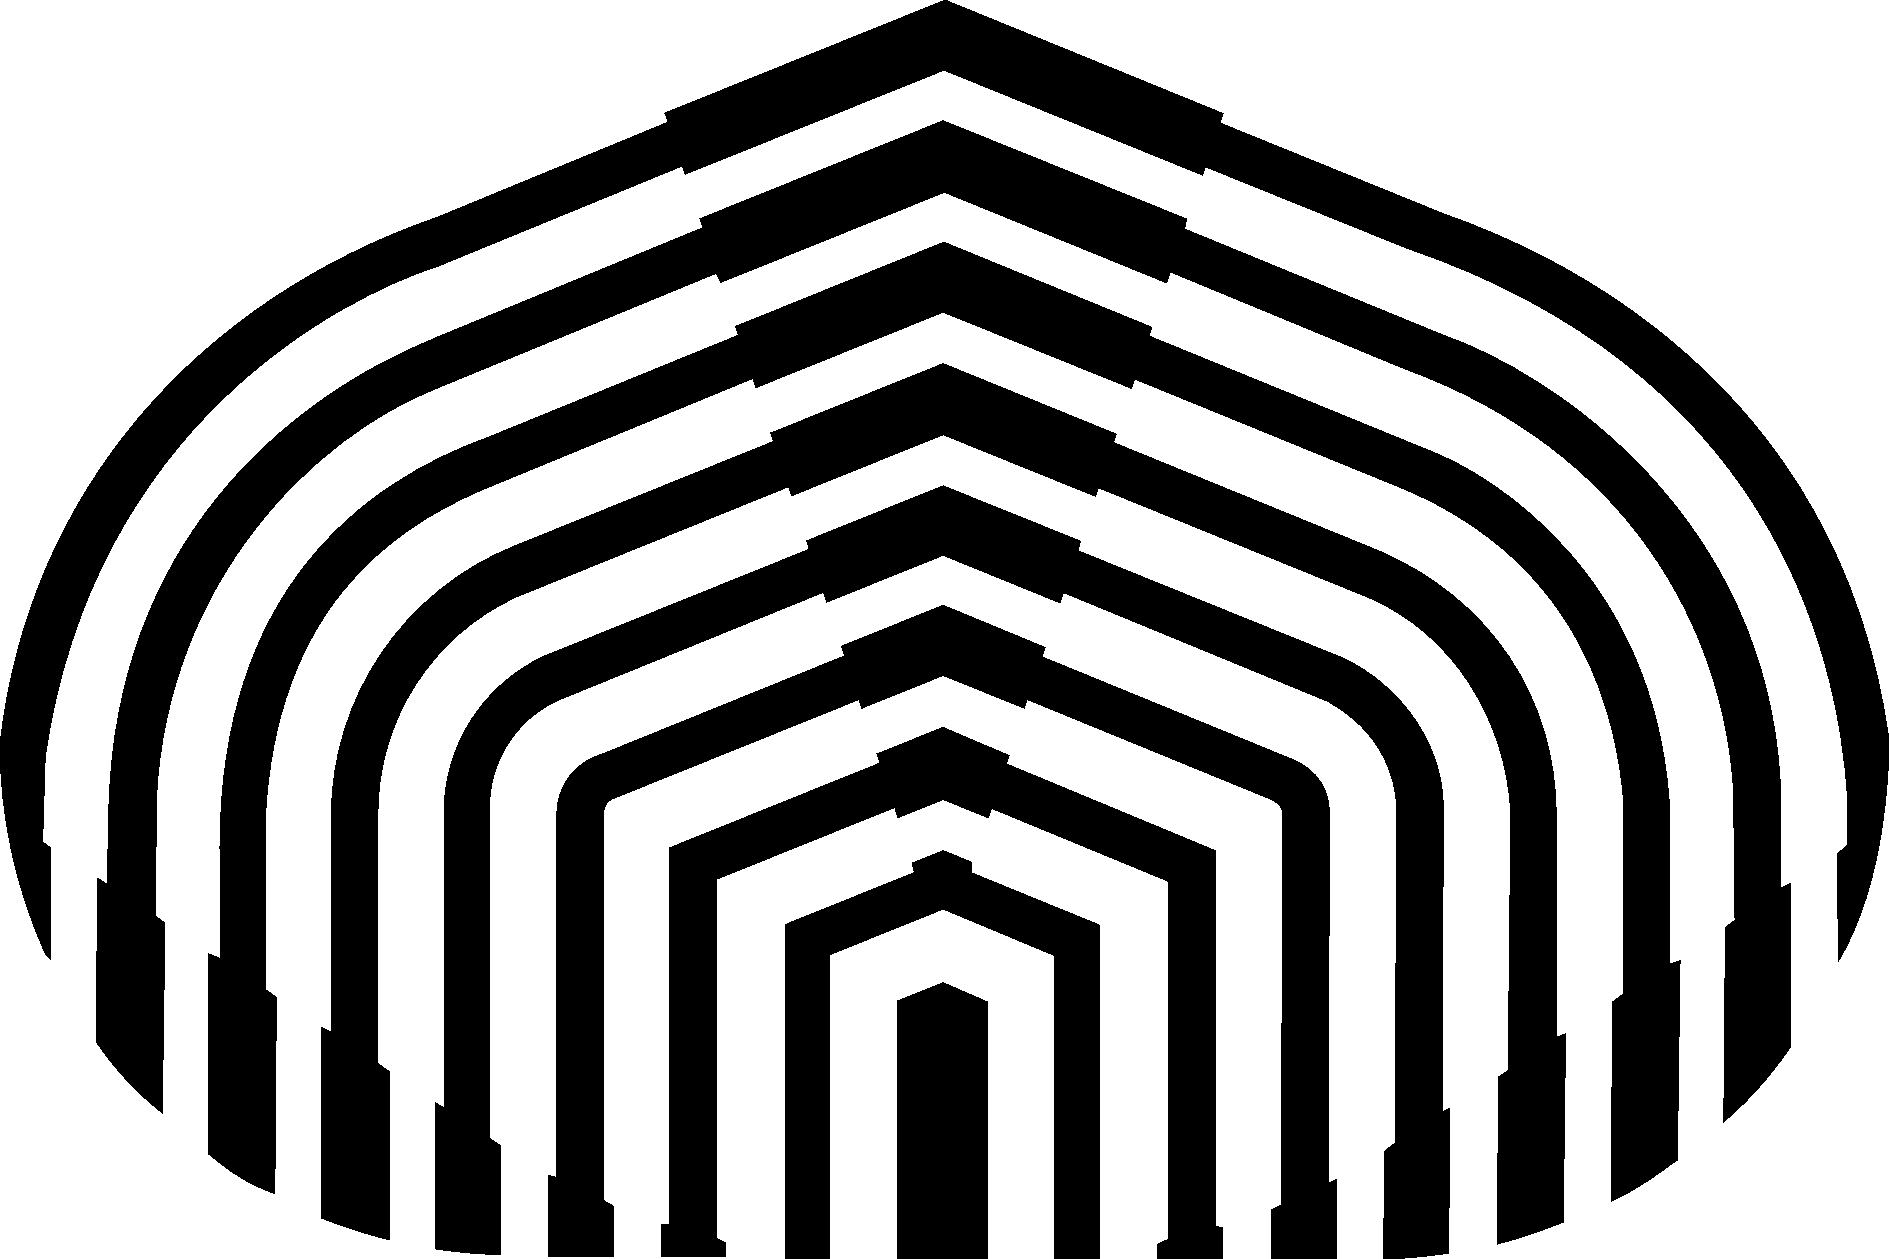
\includegraphics[scale = 0.75]{usb.png}
\end{center}
\begin{center}
\large Universidad Simón Bolívar
\end{center}
\begin{center}
 \large Diseño de Algoritmos I
\end{center}


\end{figure}


\maketitle


\thispagestyle{empty}
\newpage

\tableofcontents{}
\newpage


\section{Introducción}

\subsection{Motivación del Proyecto}
Encontrar la coloración mínima es un problema de complejidad NP. 
Sus soluciones son ampliamente aplicadas en casos de la vida real, a nombrar:
\begin{itemize}
 \item Problema de planificación de horarios
 \item Asignación de frecuencia a radios móviles.
 \item Ubicación de registros en la computadora.
 \item Análisis de datos arqueológicos y biológicos.
\end{itemize}
Por estas razones el problema de coloración mínima en un grafo se hace 
interesante hasta el punto de tratar de resolver dicho problema con 
algoritmos optimizados.

\subsection{Breve descripción del problema}
El problema se aborda con ayuda de la combinación los algoritmos 
Brelaz+Interchange y Enumeraci\'on Impl\'icita. El algoritmo de
Enumeraci\'on impl\'icita es una combinaci\'on del algoritmo propuesto por Kubale y
Jackowski y el algoritmo ``Brown's modified algorithm with look-ahead
rule'' propuesto por Peemoller, tambi\'en se tomaron ideas del algoritmo
de Brelaz.
Brelaz+Interchante es usado para encontrar un cota superior y una
cota inferior, luego el algoritmo de Enumeración Implícita usa estas
cotas para podar el \'arbol en su exploració, reducir su profundidad
y detectar cuando se ha llegado a una coloración mínima durante la
busqueda de soluciones.

\subsection{Descripción del contenido del informe}
En este informe se explica el concepto de diseño que se utilizó
para lograr el objetivo, así también como los detalles de implementación, 
instrucciones de operación, estado actual, conclusiones y referencias bibliográficas.

\section{Diseño}

\subsection{Descripción y justificación del modelo utilizado para
  representar el problema}

\subsubsection{Representación de Grafo }
Para representar el grafo en el computador se utilizar\'on arreglos de
  adyacencias, estos estan formados por un arreglo de igual tamaño al número de
  vértices del grafo, cada posici\'on del arreglo contiene la
  informaci\'on del vertice numerado con esa posici\'on, as\'i, la
  informaci\'on del v\'ertice cero esta al principio del arreglo, la del
  vertice cuatro esta en la posici\'on cuatro del arreglo... Cada
  casilla de dicho arreglo es una estructura Graph que contiene un
  apuntador a un arreglo de adyacencias, un color, un arreglo que
  llamamos color-around y una estructura Label que se define m\'as
  adelante en la secci\'on de estructuras de datos. Se decidió utilizar
  un arreglo ya que proporciona acceso constante a sus elementos.\\

\subsubsection{Vértices adyacentes}

 Para las adyacencias se podr\'ia haber utilizado una lista enlazada ya
  que cada vez que se requiere saber los adyancentes a un vértice dado
  siempre es necesario recorrerlos todos, y generar una lista de
  enlazada con los adyacentes es m\'as f\'acil y r\'apido que hacer un
  arreglo (debido a que no se sabe cuanto va a medir
  ese arreglo durante la primera lectura del archivo con la
  especificaci\'on del grafo), sin embargo, la lista enlazada podr\'ia
  inutilizar el cache del procesador, mientras que el arreglo no.\\

  \indent No se decidi\'o hacer una matriz de NxN porque en ese caso, para recorrer los
  adyacentes a un nodo, se deben recorrer inevitablemente N casillas, lo
  cual representa tiempo gastado in\'utilmente, sobre todo para grafos
  poco densos, ya que es necesario recorrer las casillas de los nodos que
  no son adyacente y las de los que son adyacentes. Debido a esto vemos
  que la estructura de arreglos de adyacencias se comporta mejor que la
  matriz de NxN para grafos poco densos e igual de bien para grafos muy
  densos. Además añadiendo un ordenamiento a los arreglos de adyacencias, cada vez que 
se necesita saber si un vértice es vecino de otro, simplemente se busca ese vértice en log(n)
utilizando búsqueda binaria.

\subsubsection{Historial de backtracks: Trace}

Debido a que el algoritmo de backtracking es iterativo no se cuenta con la pila 
para mantener un rastro del backtrack que se ha ido haciendo. Por lo tanto se decidió
utilizar un arreglo de tamaño n (número de vértices) llamado \textbf{trace} en donde 
se van poniendo los vértices coloreados a medida que el procedimiento Forward avanza en
la coloración. La traza siempre tendrá un cota hasta donde es posible leer datos confiables, 
y esta cota es la profundidad en el arbol de backtrack, es decir cuantos niveles se ha descendido 
en el árbol. La profundida se representa con la variable \textbf{depth}. Cualquier índice en la 
traza que esté después de la posición depth contendrá basura o datos que no son útiles para el 
algoritmo. 

\subsubsection{Estructura Popularity}
Esta estructura es un arreglo de tamaño ``Cota superior de Brelaz+Interchange'' y cada índice 
se corresponde a un color. En cada casilla se encuentra la popularidad de un color, es decir, 
si tenemos dos vértices coloreados con el color 4, la casilla 4 de popularity contendrá el número 2.

\subsubsection{Máximo color utilizado}

Se determina iterando desde la última casilla del arreglo Popularity hasta llegar al primer 
elemento que contenga una popularidad mayor estricta a cero. Se determina de esta manera ya que 
como popularity es de tamaño Cota Superior de Brelaz+Interchange entonces si la última casilla 
tiene un número mayor estricto que cero entonces dicho número representa el mayor color utilizado. 
Sino se busca en la penúltima casilla y así sucesivamente hasta llegar a la casilla 0.

\subsubsection{Vértice de partida para Forward y de entrada para Backwards}

La variable current-vertex se comparte entre los procedimientos Forward y Backwards. 
Ésta es la variable \textbf{r} que se utiliza en el algoritmo de Kubale y Jackowski. 

\subsubsection{Mejor coloración obtenida hasta el momento}

Se denota por el arreglo \textbf{coloring} una asignación de colores a cada índice 
el cual representa un vértice del grafo.

\subsubsection{Procedimiento de Etiquetado}

Para que un vértice $x_{k}$ sea candidato a etiquetarse, debe cumplir con tres propiedades:

\begin{enumerate}
 \item Ser adyacente a $x_{k}$
 \item Ser de menor rango que $x_{k}$
 \item Ser el de menor rango entre todos los candidatos que cumplen 
       las dos propiedades anteriores y que tengan el mismo color 
	que el vértice en cuestión.
\end{enumerate}

Una manera rápida de encontrar éste vértice candidato. Se hace de la siguiente manera: 

\begin{itemize}
 \item Se prepara un arreglo llamado colors inicializado en ceros. 
 \item Se comienza a iterar desde el principio de la traza hasta una posición  anterior al vértice
	desde donde se llama el procedimiento label. Se verifica que cumpla la propiedad 1. Luego 
	se obtiene su color, y se verifica si ese color ya se ha encontrado antes durante este proceso 
	con otro vértice. Si para tal color el arrecho colors está en cero, entonces estamos habremos 
	elegido un candidato a ser etiquetado porque es aquel que cumple con las propiedades 1,2 y 3.
\item   Seguimos el procedimiento hasta llegar a una posición anterior al vértice desde donde se llama label.
\end{itemize}
 

\subsection{Estructuras de datos y algoritmos involucrados en la aplicación}

\subsubsection{Estructuras de datos}
\begin{itemize}
 \item \textbf{Graph}: Estructura que se utiliza para representar
       un v\'ertice en los arreglos de adyacencias. El apuntador a arreglo de ints
       permite consultar el arreglo de adyacentes. El apuntador a entero llamado
       color-around es un arreglo de ints que permite saber cuáles colores
       son adyacentes al v\'ertice. La estructura Label permite saber
       si ese nodo est\'a etiquetado y a que profundidad de la rama
       explorada se encuentra. La estructura FC es un arreglo que se agrega en este 
       proyecto, el cual representa un conjunto de Colores Factibles (Feasible Colors).
	El entero adj-size es útil para saber la cantidad de vecinos de un vértice.
 \item \textbf{Label}: Tupla que consta de dos enteros, uno es un flag
       que indica si el v\'ertice esta etiquetado o no y el otro es su
       profundidad de la rama que se estaba explorando cuando fue
       etiquetado.
 \item \textbf{Tuple}: Tupla que sirve para representar los vertices con su 
       grado en el arreglo ordenado por grados que pide DSATUR.
 \item \textbf{Pair}: Pair es la estructura que retorna Dsatur.
       Clique representa la cota inferior de coloración.
       Coloring representa la cota superior.
       Members es un arreglo que contiene los miembros
       que conforman la clique máxima encontrada por el algoritmo.
 \item \textbf{Linked-Array-list}: contiene un apuntador a arreglo, un
       color, y un apuntador a un arreglo. Es utilizada en interchange 
       para guardar componentes de un grafo representadas como conjuntos
       vectoriales.
\end{itemize}
 
\subsubsection{Algoritmos involucrados}

\begin{itemize}
 \item \textbf{Dsatur+interchange}: para el ordenamiento decreciente de
       los vértices se utilizó el Algoritmo Quicksort. Los grados de
       saturación sólo se actualizan para los vértices que no han sido
       coloreados, de esta manera se ahorra costo de operaciones. El
       algoritmo recibe un argumento llamado start-point el cuál es -1
       para indicar que se quiere hayar la cota superior y recibe algún
       número mayor o igual que cero hasta el número de vértices del
       grafo cuando se quiere encontrar la clique máxima (cota
       inferior). \'Este algortimo usa las siguientes rutinas:
\begin{itemize}
 \item \textbf{get-max-degree}: función que en caso de ocurrir una
       igualdad en los números de saturación devuelve el próximo vértice
       no coloreado de grado mayor.
 \item \textbf{update-satur}: modifica estructuras de datos en vértices
       adyacentes a v(sub)i en el momento que se colorea un vértice
       v(sub)i todos los adyacentes a éste sufren un aumento de
       saturación siempre que el color utilizado no sea el de uno
       adyacente a un adyacente de v(sub)i. Si el grado de saturación de
       un elemento es -1 significa que dicho elemento ya fue
       coloreado. Por otro lado, se aprovecha de colocar en 1 la casilla
       que corresponde al color utilizado por v(sub)i indicando que 
       existe un vértice en las adyacencias del vértice con un color
       dado.
 \item \textbf{leasp-color}: retorna el menor color posible. Dado un
       vértice v(sub)i que se quiere colorear se utiliza la estructura
       color-around. Sobre ésta se itera desde el principio hasta
       conseguir alguna casilla en 0 (indicando la ausencia del color i
       en la casilla).
 \item \textbf{repeated}: algoritmo que en caso de encontrar una
       repetición de grados de saturación devuelve el próximo vértice de
       grado mayor no coloreado.
\end{itemize}
 \item \textbf{compare-vertices}: función de comparación utilizada por
       Quicksort y B\'usqueda binaria.
 \item \textbf{Degree}: prepara los vértices en una estructura
       vértice-grado llamada tupla, luego todos estos elementos se
       almacenan en un arreglo de tuplas llamado deg-vert. \'Este
       arreglo es utilizado en Enumeraci\'on impl\'icita y en Dsatur.
 \item \textbf{twoOnN}: algoritmo que cálcula la combinatoria de 2
       elementos en número colores.
 \item \textbf{interchange}: se calculan las componentes por medio de un
       DFS en los nodos. Se verifica la condición de intercambio y se
       hace el intercambio en caso de proceder.
\end{itemize}

\subsubsection{Enumeraci\'on impl\'icita}
Funci\'on que encuentra una coloraci\'on m\'inima por medio de una
estrategia de backtracking.\\

\indent Se implement\'o el algoritmo ``Brown's modified algorithm with
look-ahead rule'' de Peemoller con varias modificaciones y
correciones. Se utiliz\'o como plantilla el algoritmo generalizado de
enumeraci\'on impl\'icita propuesto por Kubale y Jackowski. Las
modificaciones al algoritmo de Peemoller fueron:
\begin{itemize}
\item El pr\'oximo v\'ertice a colorear se decide en base al grado de
      saturaci\'on, no en base al n\'umero de prevenciones y bloqueos.
\item El pr\'oximo color a usar se decide en base a la popularidad de
      ese color, no se elige el menor color posible.
\item Cuando se consigue una coloración completa los FC se vuelven a generar 
	a partir de una cota que está por debajo de todos los colores que se 
	usaron en la coloración pasada.
\item Cuando existe un color que bloquea a algún vértice no coloreado, se llama
	el procedimiento de label para etiquetar los vértices que cumplen las 
	propiedades de labeling, pero no se procede hacer backtracking a menos 
	que el vértice con el color bloqueante tenga un FC vacío.
\end{itemize}

\indent El algoritmo explora el grafo de todas las posibles particiones
de los nodos del grafo, sin embargo, por la manera en que se generan los
hijos de los nodos, podemos decir que exploran todas las posibles
coloraciones parciales y completas del grafo. La manera concreta en que
se generan los nodos del \'arbol es la que sigue:
\begin{itemize}
 \item Un nodo es v\'alido si todos los nodos
       pertenecientes a un mismo conjunto no son adyacentes entre
       s\'i. Interpretamos el hecho de que una cantidad X de
       nodos pertenezcan a un conjunto como que esos X nodos
       est\'an pintados con el mismo color.
 \item Un sucesor v\'alido de un nodo es aquel donde se ha an\~adido el
       v\'ertice con mayor grado de saturaci\'on a uno de los conjuntos de la
       partici\'on donde no sea adyacente a ning\'un vertice de ese
       conjunto, o donde se ha creado un nuevo conjunto y an\~adido el
       nodo a ese conjunto.\\
       \indent Tenemos que, por el teorema Brown de asignaci\'on de atributos
       indistingibles evitando generar soluciones redundates, se
       exploran todas las posibles coloraciones parciales y completas
       del grafo evitando por completo la redundancia de soluciones.
\end{itemize}

\indent Este grafo implic\'icito se recorre de manera iterativa como sigue:
\begin{itemize}
 \item Se encuentra una clique y cota inferior usando Brelaz. Se colorean los
       v\'ertices de esa clique.
 \item Se encuentra una cota superior aplicando Brelaz+interchange.
 \item El pr\'oximo v\'ertice a colorear ser\'a siempre el que tenga
       mayor grado de saturaci\'on.
 \item Para colorear un v\'ertice se elige del conjunto de colores que hallan
       sido usados anteriormente y que no generen una coloraci\'on
       inv\'alida, o se introduce un nuevo color. Para determinar exactamente
       en que orden se eligir\'an los colores se implementaron dos heur\'isticas.
       \begin{itemize}
	\item Se elige el color m\'as usado o m\'as popular en la coloraci\'on
	      explorada que no halla sido usado anteriormente para
	      colorear el v\'ertice que se est\'a procesando. 
	\item Se elige el color menos usado o menos popular en la
	      coloraci\'on explorada que no halla sido ya usado
	      anteriormente para colorear el v\'ertice que se est\'a
	      procesando. Sin embargo se asegura que introducir un nuevo
	      color siempre ser\'a considerado como la \'ultima opci\'on.
       \end{itemize}
       No se consideran aquellos colores que sean mayores a la cota
       superior previamente calculada. Tampoco se consideran los colores
       que hagan el conjunto de colores de alguno de los vecinos
       adyacentes al nodo procesado vac\'io (look-ahead), si esto llega
       a pasar, se aplica el algoritmo de etiquetado para look-ahead
       propuesto por Peemoller.
\item Se repiten los dos pasos anteriores hasta encontrar una
      coloraci\'on completa o hasta llegar a un nodo con conjunto de
      colores posibles vac\'io.
\item Tenemos dos posibilidades:
      \begin{itemize}
	\item Se encontr\'o una coloraci\'on completa. En ese caso se
	      guarda esta nueva coloraci\'on y se revisa si esa usa
	      tantos colores como la cota inferior, de ser ese el caso,
	      el algoritmo termina, si no, se reduce la cota superior en
	      uno y se hace backtrack hasta el primer v\'ertice
	      coloreado con el color m\'as alto usado y se aplica el
	      proceso de labeling propuesto por Peemoller.
	\item Si se lleg\'o a un v\'ertice con un conjunto de colores
	      posibles vac\'io, se aplica el procedimento de labeling de
	      Peemoller directamente.
      \end{itemize}
\item Una vez que se a aplicado labeling y se ha llegado al v\'ertice
      desde donde se reanudará la exploraci\'on, se repite todo el
      proceso desde el paso n\'umero tres. En caso de que el proceso de
      labeling no pueda conseguir un nodo desde donde resumir la
      exploraci\'on, el algoritmo retorna y devuelve la mejor
      coloraci\'on hasta el momento encontrada, que ser\'a la \'optima
      como veremos m\'as adelante.
\end{itemize}
       
\newpage
\section{Detalles de Implementación}

\subsection{Reseña de los elementos implementados, problemas encontrados y solución}

\subsubsection{Representación y Actualización Del Grafo para Brelaz+Interchange}

Para la representación del grafo el principal desafío fue poder
actualizar coloración y saturación rápidamente, incluso después de un
intercambio.

El grafo esta representado como un arreglo de listas de
adyacencias. Cada índice representa un nodo, los cuales enumeramos a
partir de cero. Cada índice del arreglo guarda el color del nodo, un
apuntador a su lista de adyacentes y un apuntador a un arreglo que
guarda la cantidad de vecinos que tienen un determinado color al que
llamaremos \textbf{color-around}, hablaremos de \textbf{color-around}
más adelante.

Las listas de adyacentes solo contienen el índice del vecino en el
arreglo de listas de adyacencias. Estas listas ameritan ser liberadas de
memoria en tiempo O(Grado del grafo).

El color se guarda como un entero, ya que también numeramos los colores
desde el cero. Para nodos no pintados, el color es -1.
color-around contiene, para el indice i, el numero de vecinos que están
coloreados con el color i. Este arreglo es tan largo como el número de
vértices de grafo.

Además de esta estructura, también mantenemos un arreglo, llamado
degree-vert, que mantiene un registro de la saturación de los nodos del
grafo. degree-vert contiene para el índice i, la cantidad de colores
distintos adyacentes al vértice i. Este arreglo también es tan largo
como nodos tenga el grafo.

El hecho de que las listas solo guarden el índice del vecino y el hecho
de que el color se guarde directamente en el arreglo con las listas de
adyacencias nos permite actualizar el color de un nodo en O(1).
color-around combinado con degree-vert nos permite actualizar la
saturación en O(grado(i)), siendo grado(i) la función que devuelve el
grado del vértice i. Cuando se colorea un nodo, basta con chequear para
cada vecino si ya tenían referencias al nuevo color del nodo, si no
tenían tales referencias se aumenta en uno(1) su grado de saturación en
degree-vert, luego se aumenta en uno(1) el numero de referencias en
color-around. Cuando se cambia el color de un nodo basta con (para cada
vecino) restar en color-around uno(1) a las referencias del color viejo,
y si llegase a cero, se disminuye la saturación en degree-vert en
uno(1), la actualización por el color nuevo es igual a cuando se colorea
un nodo por primera vez.


\subsubsection{Intercambio}

Hubo dos temas cruciales en el diseño de intercambio, uno fue la
búsqueda y representación de las componentes inducidas por los dos
colores elegidos, el otro fue el cálculo de todas las combinaciones de
dos colores del conjunto de colores adyacentes el nodo del intercambio.
Encontrar componentes en esta estructura puede lograrse, gracias a las
listas enlazadas, en O(Nodos alcanzables desde el punto de partida),
usando DFS o BFS. Nosotros elegimos DFS por su simplicidad.

Para guardar las componentes encontradas en intercambio se usa una lista
enlazada simple que contiene apuntadores a arreglos. Estos arreglos se
crean de tamaño igual a la cantidad de vértices del grafo y se utilizan
como conjuntos vectoriales (1 si el elemento esta, 0 en caso
contrario). Estos arreglos vectoriales nos permiten revisar rápidamente
si un nodo pertenece o no a una componente y llenarlos también es fácil
y rápido. Su desventaja es que ameritan que sean liberados de memoria
cuidadosamente y en tiempo O(Número de componentes).

Nunca vimos la necesidad de inducir un grafo. La exploración en un grafo
inducido la pudimos lograr discriminando que nodos examinar viendo sus
propiedades.

Para el cálculo de las combinaciones de colores ideamos un algoritmo que
solo funciona para calcular combinatorias de dos elementos, pero que
solo amerita un(1) intercambio para obtener siguiente combinación. La
desventaja de este algoritmo es que requiere de una pequeña estructura
de control para que pueda funcionar a través de varias llamadas la
función que lo contiene.

El algoritmo se basa en el hecho de que, una vez que se combina un
elemento con todos los demás elementos de su conjunto, se puede dejar de
considerar ese elemento en las combinaciones posteriores, y se puede
operar recursivamente sobre lo que sobra del conjunto.


\subsubsection{Enumeración Implícita}
El algoritmo se implemento siguiendo el esquema propuesto por Kubale y
Jackowski, por lo que el algoritmo dividido en dos funciones principales,
Forward y backwards.\\

\indent Debido a que se elige el pr\'oximo v\'ertice a colorear en base al grado de
saturaci\'on, tomamos muchas ideas del algoritmo de Brelaz para la
implementaci\'on de este algoritmo. De hecho, lo que hace la funci\'on
Forward es, b\'asicamente, ir coloreando el grafo en base al grado de
saturaci\'on, siempre asegurandose de no repetir soluciones o explorar
varias veces una misma rama.\\

\indent Durante la implementaci\'on del algoritmo de Brelaz se decidi\'o
que en las deciciones de dise\~no se sopesar\'ia m\'as la eficiencia en
tiempo que en espacio, ya que el algoritmo no consume mucha memoria per
se y se buscaba una implementaci\'on r\'apida.\\

\indent Esta desici\'on gener\'o muchos arreglos y estructuras de datos
de control para guardar la informaci\'on necesaria para calcular y
actualizar los grados de saturaci\'on r\'apidamente.\\

\indent Como ya se mencion\'o, debido a la heur\'istica de elecci\'on
del pr\'oximo v\'ertice se tomaron muchas ideas de la implementaci\'on
de Brelaz permitieron hacer una funci\'on de forward muy
r\'apida y concisa. Sin embargo, la cantidad de estructuras de datos que
se usaron para llevar un control de la saturaci\'on de los v\'ertices se
volvieron una carga bastante grande a la hora de usarlas en una
implementaci\'on por backtracking en vez de greedy, ya que as\'i como se
actualizan durante el Forward, se deben actualizar durante el backwards,
lo cual implica que se gasta tiempo actualizando las estructuras durante
cada uno de los backtracks.\\

\indent Para representar el conjunto FC se a\~nadieron estructuras a los
v\'ertices en los arreglos de adyacencias. La estructura Graph ahora
tiene un arreglo de enteros que representa en forma de conjunto
vectorial la pertenencia de un color al conjunto de colores v\'alidos
para un v\'ertice, se utiliza un entero para indicar cual es el color
m\'as grande que se puede usar. Durante el Forward estos se sobreescriben, ya que la
informaci\'on que tuvieran previamente no es representativa de nada ya
que se est\'a explorando una nueva rama. Hay que agregar que durante la
generaci\'on del FC se aplica look-ahead para tratar de reducir su
cardinalidad, tambien se utiliza el procedimiento de etiquetado
propuesto por Peemoller para el look-ahead.\\

\indent Para representar el conjunto CP se us\'o el procedimiento de labeling de
Peemoller. Se agrego a la estructura Graph un atributo Label que indica
si el nodo est\'a etiquetado o no y cual es su profundidad en la rama
explorada actualmente. Con esto se puede buscar f\'acilmente el
etiquetado de menor rango.

\subsubsection{Bugs encontrados}
La fase de debuggin fue bastante larga ya que se cometió el error de diseño 
de hacer dos funciones Backwards y Forwads que compartiesen datos muy delicados 
para la obtención de resultados. Ambas funciones propiciaban efectos de borde a estos 
datos compartidos, y cualquier error cometido en la modificación de estos datos hacía 
que el algoritmo simplemente nunca llegara a una solución o fallara en el intento. 
Luego de solucionar todos estos problemas de dependencia de datos, se arreglaron 
algunos ``leaks'' de memoria (memoria no liberada). 
\newpage

\section{Instrucciones de Operación}

\subsection{Código fuente de aplicación}
El código fuente se puede conseguir en el archivo tar.gz que viene con
éste informe.

\subsection{Descripción detallada de como compilar y correr la aplicación}

\subsection{¿Cómo descomprimir el archivo tar.gz?}
En una cónsola de linux se debe ejecutar el siguiente comando:
\begin{verbatim}
 tar -vzxf proyecto2-Fundaro-Jaber.tar.gz
\end{verbatim}
A continuación se crea una carpeta llamada proyecto2 dónde se encuentran
los archivos fuentes del proyecto.


\subsection{¿Cómo compilar?}
En una cónsola de linux debe dirigirse a la carpeta donde estan los
archivos fuentes.//
\indent Si desea compilar el algoritmo DSATUR+ haga el siguiente comando:
\begin{verbatim}
 make mas
\end{verbatim}

\indent Si desea compilar el algoritmo DSATUR* haga el siguiente comando:
\begin{verbatim}
 make estrella
\end{verbatim}

En caso de querer borrar los archivos generados por la compilación
proceda a hacer:
\begin{verbatim}
 make clean
\end{verbatim}

\subsection{¿Cómo ejecutar?}
En la carpeta de archivos fuentes se provee de un script llamado
script.sh. Si se quieren ejecutar todas las instancias el comando que
debe ejecutar es:
\begin{verbatim}
 ./script.sh <resultado>
\end{verbatim}

Si desea ejecutar solo aquellas instancias donde las cotas generadas por
DSATUR no son iguales, ejecute el comando:
\begin{verbatim}
 ./script.sh -c <resultado>
\end{verbatim}

<resultado> en este caso es el nombre del archivo donde se guardaran los
resultados de la corrida. Si se quiere, éste archivo puede recibir
cualquier nombre diferente a resultado.

Si se quiere ejecutar una instancia particular se procede con el
siguiente comando:

\begin{verbatim}
 ./main < instancias/instancia-particular
\end{verbatim}

\newpage
\subsection{¿Cómo interpretar resultados?}
Cada instancia arroja un resultado con la siguiente estructura:
\begin{verbatim}
1 ---- 20-0,7-1.col -----
2 Resultados de Brelaz+interchange 
3 Cota superior = 9                
4 Cota inferior = 8                
5 ------------------               
6 Enumeración implícita            
 Mejor Coloración Actual --> Cota_superior - 1
. ....
. ....
. Mejor Coloración Actual --> Cota_inferior
7 Numero cromatico: 9              
8 Backtracks: 3                    
9 Vertice --> Color                
   1 --> 1                          
   2 --> 6                          
   3 --> 2                          
   4 --> 3                          
   5 --> 3                          
   6 --> 7                          
   7 --> 4
   8 --> 8
   9 --> 2
   10 --> 5
   11 --> 8
   12 --> 9
   13 --> 6
   14 --> 2 
   15 --> 5
   16 --> 7
   17 --> 1
   18 --> 4
   19 --> 4
   20 --> 8
10 Tiempo en segundos de ejecución del programa: 0.0262
\end{verbatim}
Explicación de cada línea:
\begin{enumerate}
 \item Nombre de la instancia, el primer número indica la cantidad de vértices, el segundo la densidad y el tercero el número de archivo.
 \item Indicador de algoritmo.
 \item Coloración arrojada por Brelaz-Interchange.
 \item Cota inferior. Clique máxima encontrada al aplicar Brelaz-Interchange N veces.
 \item Indicador de algoritmo. (Enumeración Implícita)
 \item A continuación líneas que van informando del progreso del
       algoritmo de backtracking.
 \item Número cromático encontrado por enumeración implícita.
 \item Cantidad de backtracks realizados por el algoritmo.
 \item A partir de la l\'inea 10 tenemos la coloraci\'on encontrada.
 \item Tiempo en segundos según función provista en el proyecto.
\end{enumerate}
Si Brelaz-Interchange arroja una cota superior igual a la inferior
entonces el algoritmo de enumeración implícita no se ejecuta.

\section{Estado Actual}
\subsection{Indicación del estado final de la aplicación}
La aplicación en estos momentos está totalmente funcional. Las tablas 
reflejan que el algoritmo DSATUR+ es mucho más efectivo que DSATUR* debido 
a la heurística utilizada para elegir el próximo color a utilizar.

\section{Otros}
\subsection{Demostración formal de Enumeración Implícita}
Dado que es un algoritmo de backtracking, se empezar\'a por definir el
grafo impl\'icito.\\
\indent El grafo impl\'icito es el todas las posibles particiones de
nodos del grafo, definimos el grafo impl\'icito como sigue:
\begin{itemize}
 \item Un nodo v\'alido es aquel que contiene una partici\'on de los
       v\'ertices del grafo. 
 \item Un hijo v\'alido es aquel donde se ha agregado un v\'ertice del
       grafo a uno de los conjuntos de la partici\'on, siempre y cuando
       ese v\'ertice no halla sido agregado antes a ninguna de las
       particiones de esa rama del \'arbol.
 \item Un hijo v\'alido tambi\'en puede ser una partici\'on a la cual se
       le ha agregado un conjunto un v\'ertice del grafo, siempre y
       cuando ese v\'ertice no halla sido agregado antes a ninguna de
       las particiones de esa rama del \'arbol.
\end{itemize}
\indent Una partici\'on puede ser interpretada como una coloraci\'on (no
necesariamente v\'alida) donde cada conjunto de la partici\'on
representa un color \'unico y donde el hecho de que un nodo pertenezca a
un conjunto se interpreta como que ese nodo est\'a coloreado del color
que representa la partici\'on.
Por lo tanto:
\begin{itemize}
 \item Dado que el \'arbol contiene todas las particiones posibles,
 toda coloracion v\'alida existe en alguna hoja del \'arbol.
 \item Dado que cualquier soluci\'on \'optima es una coloraci\'on
 v\'alida, \'esta debe estar en el \'arbol.
\end{itemize}

\indent Se establece una cota superior buscando una coloraci\'on
v\'alida.\\
\indent Se establece una cota inferior buscando una clique en el grafo.\\
\indent Cuando se genera el FC, se excluyen los colores que genera\'ian
una coloraci\'on inv\'alida, tambi\'en se excluyen colores que
generar\'ian una coloraci\'on con m\'ayor o igual n\'umero de colores
la cota superior.\\
\indent Existen dos formas de elegir el pr\'oximo color:
\begin{itemize}
 \item Eligiendo el color que m\'as se ha usado en la coloraci\'on
       parcial hasta ahora generada.
 \item Eligiendo el color que menos se ha usado en la coloraci\'on
       parcial hasta ahora generada. Siempre asegurando que se elija
       introducir un color nuevo de \'ultimo.
\end{itemize}
\indent Cada vez que se encuentra una coloraci\'on completa, se
actualiza la cota superior al n\'umero de colores usados por esa nueva
coloraci\'on.\\
\indent El CP contiene s\'olo nodos coloreados adyacentes al nodo desde
donde se hace el backtrack. M\'as a\'un, s\'olo tiene aquellos
adyacentes al nodo actual que tienen m\'inimo rango entre los adyacentes
de su color.\\
Por lo tanto se tiene que:
\begin{itemize}
 \item Si se usa la primera estrategia para elegir el pr\'oximo color,
       introducir un color nuevo siempre sera la \'ultima opci\'on, ya que
       siempre ser\'a el que tiene menos popularidad. Si se utiliza la segunda
       estrategia, siempre se eligir\'a un nuevo color de \'ultimo ya que es
       parte de la definici\'on del criterio.\\
 \item Si se hace backtrack porque el FC es igual a vac\'io cambiar el
       color de un nodo no adyacente al nodo actual no cambiar\'a su FC.\\
 \item Si se hace backtrack porque se lleg\'o a una coloraci\'on
       completa, se desea una coloraci\'on con menos colores, por lo que se
       debe cambiar el color del primer nodo (rango mínimo) con el m\'aximo color usado. El nodo
       con el m\'aximo color usado debe tener un FC={<maximo\_color>}
       (debido a la forma en la que se eligen los colores), por el
       punto anterior, uno de sus vecinos coloreados debe cambiar.
 \item Dado que se incluyen todos los nodos que podr\'ian inducir un
       cambio en el color del nodo del backtrack, recolorear cualquier otro
       nodo llevar\'ia a un FC=vac\'io, por lo que no se excluyen soluci\'ones
       v\'alidas en la construcci\'on del CP.
 \item Dado que cuando se genera el FC, solo se incluyen colores que
       generan coloraciones v\'alidas menores a la cota superior, no se
       excluyen soluci\'ones \'optimas en la construcci\'on de FC.
 \item No se excluyen soluciones \'optimas durante la exploraci\'on del
       grafo, y ya que se exploran todas las soluciones no podadas, se
       debe explorar una soluci\'on \'optima necesariamente.
\end{itemize}

El algoritmo se detiene cuando encuentra una coloraci\'on con tantos
colores como la cota inferior. Esto indica que la coloraci\'on debe ser
optimal, ya que no pueden existir coloraciones con menor n\'umero de
colores que la cota inferior.

Si el algoritmo nunca encuentra una coloraci\'on con tantos colores como
la cota inferior, devolver\'a la mejor coloraci\'on encontrada. Dado que
el algoritmo devuelve la mejor soluci\'on encontrada, y dado que el
algoritmo explora una soluci\'on \'optima, la mejor soluci\'on
encontrada debe ser la \'optima encontrada.


\subsection{Tabla de resultados}
A continuaci\'on se presentan las tablas de resultados. Se dar\'an ahora
las instrucciones para interpretar estas tablas y las descripciones de
las instancias con las que se experiment\'o.

\subsubsection{Leyenda de las tablas de resultados}
\indent En la cabezera de la tabla se encuentra el tipo de instancia
seguida de una expresi\'on regular encerrada entre par\'entesis
que indica el nombre que tienen todos los archivos pertenecientes
a dicha instancia.

\indent Los nombres de las instancias est\'an escritos de la siguiente forma:
\begin{itemize}
 \item Primero, entre par\'etesis, el n\'umero de nodos y la densidad
       separados por un espacio. En caso de no conocerse la densidad se
       pondr\'a el n\'umero de lados precedido por un '?'
 \item Despu\'es de esta informaci\'on est\'a el nombre del archivo con
       la instancia probada.
 \item Debajo de los nombres de las instancias tenemos los campos donde
       se encuentran los resultados de los algoritmos analizados.
\end{itemize}

\indent Para el algoritmo DSATUR+Interchange:
\begin{itemize}
 \item El primer n\'umero es la cantidad de colores que utiliz\'o el
       algoritmo para la instancia dada.
 \item El segundo n\'umero esta seguido siempre por una letra 'k' y es el n\'umero crom\'atico de la
       instancia. En caso de que no se conozca el n\'umero crom\'atico,
       se colocar\'a un '?'. Si se conoce el n\'umero crom\'atico gracias a
       referencias externas y no debido a la salida del algoritmo de
       enumeraci\'on impl\'icita, se colocar\'a un '*' al final del
       mismo.
 \item Por \'ultimo tenemos el tiempo en segundos que tard\'o el algorimo en
       encontrar la soluci\'on. Si el tiempo que tard\'o el algorimo es
       menor a 0,01 segundos, se indicar\'a que el algoritmo tard\'o
       cero segundos. Solo se colocan dos cifras decimales para los tiempos.
\end{itemize}

\indent Para el algoritmo DSATUR* y DSATUR+ (Enumeraci\'on impl\'icita):
\begin{itemize}
 \item El primer n\'umero es el n\'umero crom\'atico \'optimo
       determinado por el algoritmo.
 \item El segundo n\'umero esta seguido siempre por una letra 'b' y es
       el n\'umero de backtracks que hizo el algoritmo mientras buscaba
       la soluci\'on.
 \item Por \'ultimo tenemos el tiempo en segundos que tard\'o el algorimo en
       encontrar la soluci\'on. Si el tiempo que tard\'o el algorimo es
       menor a 0,01 segundos, se indicar\'a que el algoritmo tard\'o
       cero segundos. Solo se colocan dos cifras decimales para los
       tiempos.
 \item En caso de que el algoritmo halla tardado m\'as de 5 minutos, el
       campo s\'olo tendr\'a el texto ``Tiempo excedido''.
\end{itemize}

\indent Las instancias en las cuales se ejecut\'o el algoritmo de
enumeraci\'on impl\'icita tienen su nombre en negritas.
\indent Aquellas instancias para las cuales Brelaz+Interchange estan
tienen su nombre en letra cursiva.
\indent Aquellas instancias que tardar\'on m\'as de 5 minutos tienen el
texto ``Tiempo excedido'' en letra roja en el campo del algoritmo de
enumeraci\'on impl\'icita.
\indent Aquellas instancias donde el algoritmo de enumeraci\'on
impl\'icita encontr\'o una mejor soluci\'on que Brelaz+Interchange
tienen un fondo amarillo.

\subsubsection{Resumen de resultados}
Para el algoritmo DSATUR+:\\
\textbf{Instancias para las cuales el algoritmo DSATUR+ se activa}
\begin{itemize}
 \item 12-0,3-3.col
 \item 12-0,5-3.col
 \item 14-0,5-2.col
 \item 14-0,5-3.col
 \item 16-0,5-3.col
 \item 18-0,3-3.col
 \item 18-0,5-1.col
 \item 20-0,1-2.col
 \item 20-0,5-2.col
 \item 20-0,7-1.col
 \item fpsol2.i.1.col
 \item fpsol2.i.2.col
 \item fpsol2.i.3.col
 \item le450\_15a.col
 \item le450\_15b.col
 \item le450\_15c.col
 \item le450\_15d.col
 \item le450\_25c.col
 \item le450\_25d.col
 \item le450\_5a.col
 \item le450\_5b.col
 \item le450\_5c.col
 \item le450\_5d.col
 \item miles1000.col
 \item miles1500.col
 \item myciel3.col
 \item myciel4.col
 \item myciel5.col
 \item myciel6.col
 \item myciel7.col
 \item queen6\_6.col
 \item queen7\_7.col
 \item queen8\_8.col
 \item queen8\_12.col
 \item queen9\_9.col
 \item queen10\_10.col
 \item queen11\_11.col
 \item queen12\_12.col
 \item queen13\_13.col
 \item queen14\_14.col
 \item queen15\_15.col
 \item queen16\_16.col
 \item school1.col
 \item school1\_nsh.col
\end{itemize}
\indent Total:\textbf{44}\\

\textbf{Instancias que tardan mas de 5 minutos}
\begin{itemize}
 \item fpsol2.i.1.col
 \item fpsol2.i.2.col
 \item fpsol2.i.3.col
 \item le450\_15a.col
 \item le450\_15b.col
 \item le450\_15c.col
 \item le450\_15d.col
 \item le450\_25c.col
 \item le450\_25d.col
 \item le450\_5a.col
 \item le450\_5b.col
 \item le450\_5c.col
 \item le450\_5d.col
 \item myciel6.col
 \item myciel7.col
 \item queen8\_12.col
 \item queen9\_9.col
 \item queen10\_10.col
 \item queen11\_11.col
 \item queen12\_12.col
 \item queen13\_13.col
 \item queen14\_14.col
 \item queen15\_15.col
 \item queen16\_16.col
 \item school1.col
 \item school1\_nsh.col
\end{itemize}
\indent Total:\textbf{26}\\

\textbf{Instancias para las cuales el algoritmo DSATUR+ da mejores resultados que Brelaz+Interchange}
\begin{itemize}
 \item 12-0,5-3.col
 \item 18-0,3-3.col
 \item queen6\_6.col
 \item queen7\_7.col
 \item queen8\_8.col
\end{itemize}
\indent Total:\textbf{5}\\

\textbf{Resumen}
\begin{itemize}
 \item 66 instancias probadas.
 \item 40 instancias resueltas
 \item 26 instancias no resueltas.
 \item 22 instancias resueltas por Brelaz+Interchange.
 \item 18 instancias resueltas por DSATUR+.
 \item 5 instancias donde DSATUR+ mejora la cota superior de
       Brelaz+Interchange.
 \item 35 instancias donde la cota superior propuesta por
       Brelaz+Interchange era el n\'umero crom\'atico.
\end{itemize}
\indent Porcentaje de instancias resuelas: \textbf{60,6\%}

\subsubsection{Descripci\'on de instancias}
\begin{itemize}
 \item \textbf{Grafos aleatorios usados en el proyecto 1}: son los
       grafos generados aleatoriamente en el proyecto 1 para los cuales
       Brelaz+Interchange arrojaba cotas superior e inferior distintas.
 \item \textbf{Grafos de asignaci\'on de registros}: grafos usados para
       la asignaci\'on de registros a variables durante la ejecuci\'on
       de programas.\\
       http://mat.gsia.cmu.edu/COLOR/instances.html#XXREG
 \item \textbf{Grafos de relaciones de personajes literarios}: cada nodo
       representa un personaje de una obra literaria. Dos nodos estan
       conectados si esos dos personajes se encuentran en el libro.\\
       http://mat.gsia.cmu.edu/COLOR/instances.html#XXSGB
 \item \textbf{Grafo de temporada de f\'utbol americano}: cada nodo
       representa un equipo universitario de f\'utbol americano. Dos
       nodos est\'an conectados si esos dos equipos se enfrentaron
       durante la temporada.\\
       http://mat.gsia.cmu.edu/COLOR/instances.html#XXSGB
 \item \textbf{Grafos geom\'etricos}: cada nodo representa una ciudad de
       los Estado Unidos, dos nodos est\'an conectados el costo
       distancia/gasolina entre las ciudades es lo suficientemente
       peque\~no. El criterio para decidir que tan peque\~no es
       suficientemente pequen\~no no lo conocemos.\\
       http://mat.gsia.cmu.edu/COLOR/instances.html#XXSGB
 \item \textbf{Grafos del problema de las N reinas}: cada nodo
       representa un escaque en un tablero de ajedrez. Dos nodos est\'an
       conectados si alguna l\'inea de escaques horizontal, vertical o
       diagonal los une.\\
       http://mat.gsia.cmu.edu/COLOR/instances.html#XXSGB
 \item \textbf{Grafos de planificaci\'on de clases}: cada nodo
       representa una clase. Dos nodos est\'an conectados si esas clases
       se dictan al mismo tiempo.
       http://mat.gsia.cmu.edu/COLOR/instances.html#XXSCH
 \item \textbf{Grafos de Mycielski}: grafos basados en la
       Transformaci\'on de Mycielski. Estos grafos tienen clique
       m\'axima de dos pero n\'umero crom\'atico creciente.\\
       http://mat.gsia.cmu.edu/COLOR/instances.html#XXMYC
 \item \textbf{Grafos de Leighton}: grafos con n\'umero crom\'atico
       asegurado y n\'umero de nodos constante. El n\'umero al final del
       nombre del archivo es el n\'umero crom\'atico del grafo. Estos
       grafos est\'an descritos en detalle en:
       \begin{verbatim}
	F.T. Leighton.	
	Journal of Research of the National Bureau of Standards,  
	vol. 84, no. 6,  Nov-Dec 1979, pp 489-505.
       \end{verbatim}
       http://mat.gsia.cmu.edu/COLOR/instances.html#XXLEI
\end{itemize}


\newpage

\section{Conclusiones y recomendaciones}
El algoritmo propuesto de backtracking iterativo resulta ser 
útil para resolver la mayoría de las instancias donde Brelaz+Interchange 
tardan más del tiempo esperado. Sin embargo, cuando las densidades son muy altas 
el algoritmo tarda mucho tiempo en converger, y cuando decimos mucho tiempo nos referimos 
a que excede el tiempo límite de 5 minutos. Es necesario entonces agregar nuevas optimizaciones 
al algoritmo para así conseguir tiempos más bajos de solución. 

Como muestran los resultados la técnica del labeling no logró solucionar todas las instancias
propuestas. En muchas, el número de backtracks era tan alto que el algoritmo 
nunca logró converger. Sin embargo las instancias que se corrieron en el proyecto 
pasado se lograron resolver con la coloración óptima.


\section{Referencias Bibliográficas}
\begin{itemize}
 \item http://nicolas-lara.blogspot.com/2009/01/permutations.html (consultada el 17-02-10)
 \item http://en.wikipedia.org/wiki/Petersen-graph (consultada el 17-02-10)
 \item Meza Oscar, Ortega Maruja. “Grafos y Algoritmos”. Editorial Equinoccio, Universidad Simón Bolívar. 2007. ISBN 980-237232-3
 \item Brélaz 1979 Daniel Brélaz. «New Methods to Color the Vertices of a Graph», Communications of the ACM 22-4, 1979, 251-256
 \item Marek Kubale & Boguslaw Jackowski. ``A Generalized Implicit Enumeration Algorithm for Graph Coloring''. Communications of the ACM April 1985 Volume 28, Number 4.
 \item Jurgen Peemoller. ``A correction to Brelaz's modification of Brown's coloring algorithm''. Communications of the ACM, April 1983 Volume 26 
	Number 8.
\end{itemize}

\end{document}

